\documentclass[10pt]{article}
\usepackage{icmlko}

\icmlmeta{IP 파운데이션 월드모델}{127}{검증은 자기가 본 세계까지만 말한다}{노트 126은 시간이었고 이번은 종류다 --- 태거가 배운 레코드 안에서는 맞고 다른 종류 앞에서 무너진다}

\begin{document}

\twocolumn[
\icmlheader

\begin{abstract}
노트 126의 F8은 ``병목은 축''이라 했고 F11은 ``한 도메인에만 있는 축은
도움이 안 된다''고 했다. 남는 처방은 하나 --- \textbf{전 도메인이 공유하는
축의 빈칸을 메운다.} 노트 124가 그 빈칸을 세어 놓았고(팝업 380건 중 축이
매겨진 것 95건) ``매기면 75건이 322건이 된다''고 적었다. 그래서 태거를
만들었다. \textbf{먼저 노트 124의 산수를 고친다.} 빈 260건은 거의 전부
organizer\_claim(247)과 media\_estimate(13)이고, 그 둘은 \emph{계수 방법
필터가 이미 걸러 내고 있다.} 축만 매겨서 들어오는 것은 \textbf{17건}이다.
322이라는 숫자는 태깅이 아니라 \emph{계수 필터를 푸는 것}을 전제한 값이었고,
그건 다른 질문이다. \textbf{태거는 만들었고 작동한다.} 기획서 글에서 열 축을
되찾는데, 교차검증($n$=95, 5겹 $\times$ 12회) $\rho$가 체험 밀도 $+$0.58 ·
포토존 $+$0.54 · 굿즈 규모 $+$0.52부터 타깃 폭 $+$0.09까지 갈린다. 라벨은
한 번도 안 본다(코드로 강제). \textbf{그런데 다른 종류의 레코드에 대면
무너진다.} 학습은 내부 레코드(계약서에서 뽑은 것)로 했고 적용 대상은 시장
레코드(기사에서 뽑은 것)다. 축을 비워 둔 채로는 팝업 $\rho$ $+$0.4562인데
자동 태깅을 채우면 \textbf{$+$0.1150}으로 무너진다. 같은 종류 안에서만 재는
교차검증은 이걸 못 잡는다. \textbf{노트 126과 같은 모양이다} --- 거기서는
검증 창 \emph{뒤}에 오는 변화를 못 봤고 여기서는 검증 모집단 \emph{밖}의
글을 못 본다. 마지막으로 표본을 넓힌 값을 분해했다. 분모를 59건에 고정하면
$+$0.3688이 $+$0.4495로 오르는데, \textbf{그 값은 레코드가 늘어서가 아니라
팝업이 학습 풀에 들어가서 생긴 것이다} --- 팝업을 학습에서 빼면 오히려
$+$0.3244로 내린다.
\end{abstract}
]

\begin{figure}[t]
\centering
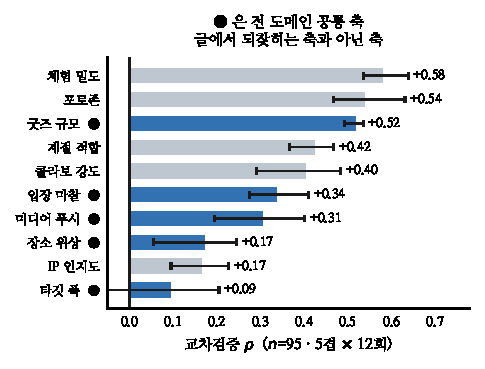
\includegraphics[width=\columnwidth]{figs/tagger.pdf}
\caption{축마다 글에서 되찾히는 정도가 다르다. 막대는 12회 반복의 평균,
수염은 90\% 구간. ● 은 전 도메인 공통 축 다섯.}
\end{figure}

\section{먼저 노트 124의 산수를 고친다}

노트 124는 팝업 축이 빈 260건을 세고 ``매기면 75건이 322건''이라 적었다.
저장소를 열어 계수 방법별로 갈라 보니 조건이 하나 빠져 있었다.

\begin{table}[t]
\centering\tsize
\caption{빈 축은 계수 방법과 거의 완전히 겹친다.}
\begin{tabular}{lrrr}
\toprule
계수 방법 & 전체 & 축 매김 & 축 빔 \\
\midrule
entry & 54 & 45 & 9 \\
participation & 37 & 29 & 8 \\
unknown & 20 & 17 & 3 \\
exposure & 5 & 4 & 1 \\
\midrule
\textbf{organizer\_claim} & \textbf{247} & \textbf{0} & \textbf{247} \\
\textbf{media\_estimate} & \textbf{13} & \textbf{0} & \textbf{13} \\
\bottomrule
\end{tabular}
\end{table}

\claimx{\textbf{현행 파이프라인은 계수 방법이 entry · participation인 것만
쓴다.} 그 안에서 축이 빈 것은 \textbf{17건}뿐이다. 260건 대부분은 태깅
이전에 \emph{계수 필터}에서 이미 빠져 있다. 노트 124의 322은 ``축을
매기고 \emph{또} 계수 필터를 푼다''를 전제한 값이었고, 그건 태깅이 아니라
\textbf{라벨 품질} 문제다.}{노트 124가 틀린 것은 결론이 아니라 산수다.
``축이 260건 비어 있다''는 여전히 맞다.}

\section{태거는 만들었고, 작동한다}

기획서 쪽 글만 읽는다 --- 콘셉트 · 브랜드명 · 체험 요소 · 프로모션 ·
연출 태그 · 장소 · 문서 제목과 종류. 다국어 문장 임베딩을 24차원으로 줄이고
세는 것들(체험 요소 개수, 평수, 운영일수, 장소 등급 등)을 붙여 축마다
능형으로 맞춘다.

\claimx{\textbf{태거는 라벨을 한 번도 보지 않는다.} 레코드에서 ``outcome''
키를 아예 지우고 넘긴다(\texttt{PLAN\_ONLY}). 노트 87과 117이 라벨 누수로
두 번 뒤집힌 뒤로는 규약을 코드로 강제한다.}{누수의 다른 경로 --- 예컨대
문서 제목에 실적이 적힌 경우 --- 는 따로 안 봤다.}

되찾히는 정도가 축마다 크게 다르다. 체험 밀도 $+$0.58 · 포토존 $+$0.54 ·
굿즈 규모 $+$0.52 · 계절 적합 $+$0.42는 쓸 만하고, 장소 위상 $+$0.17 ·
IP 인지도 $+$0.17 · 타깃 폭 $+$0.09는 사실상 못 맞힌다. 반복 표준편차가
0.015$\sim$0.086이니 이 순서 자체는 믿을 만하다.

\begin{figure*}[t]
\centering
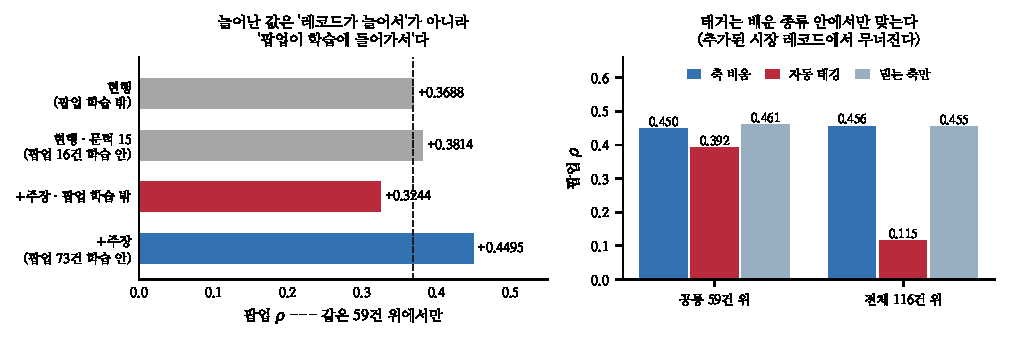
\includegraphics[width=\textwidth]{figs/expand.pdf}
\caption{왼쪽 --- 같은 59건 위에서만 비교하면 늘어난 값의 출처가 갈린다.
오른쪽 --- 태거를 다른 종류의 레코드에 대면 무너진다.}
\end{figure*}

\section{그리고 다른 종류의 레코드 앞에서 무너진다}

빈 축이 있는 레코드는 거의 전부 \emph{시장 레코드}(MKT---)다. 기사에서
뽑은 것이고, 태거가 배운 내부 레코드(계약서에서 뽑은 것)와 글의 결이 다르다.
그리고 시장 레코드 쪽에는 사람이 매긴 축이 하나도 없어서 \textbf{거기서
직접 잴 방법이 없다.} 그래서 하네스로 간접으로 쟀다 --- 축을 채운 판과
마스크로 비운 판을 나란히 붙인다.

\begin{table}[t]
\centering\tsize
\caption{계수 필터를 푼 189건에서. 채점 대상은 후행 116건.}
\begin{tabular}{lrr}
\toprule
& 축 관측률 & 팝업 $\rho$ \\
\midrule
축 비움 (마스크 0) & 0.43 & $+$0.4562 \\
\textbf{자동 태깅으로 채움} & 1.00 & \textbf{$+$0.1150} \\
믿는 축만 ($\rho>.3$) & 0.54 & $+$0.4551 \\
\bottomrule
\end{tabular}
\end{table}

\claimx{\textbf{자동 태깅이 점수를 무너뜨린다.} 축을 비워 두면 $+$0.4562인데
채우면 $+$0.1150이다. 그런데 \emph{원래 있던 59건 위에서만} 재면 $+$0.3917로
멀쩡하다. 무너지는 것은 새로 들어온 시장 레코드 쪽이다. 태거는 배운 종류
안에서만 맞는다.}{시장 레코드에 참값이 없으니 ``태그가 틀렸다''를 직접
확인한 것은 아니다. 하네스를 통한 간접 증거다.}

\claimx{\textbf{교차검증은 이것을 못 잡는다.} $n$=95 내부 레코드 안에서
12회 반복해도 나오는 것은 ``내부 레코드에서 $\rho$ 0.35''뿐이다. 다른
모집단에서 얼마나 맞는지는 그 절차가 대답할 수 있는 질문이 아니다.}{믿는
축만 채우면($\rho>.3$) $+$0.4551로 비움과 같아진다. 즉 잘 되찾히는 축은
해가 되지도 않지만 도움도 안 된다.}

\section{노트 126과 같은 모양이다}

\begin{table}[t]
\centering\tsize
\caption{검증이 보지 못하는 두 방향.}
\begin{tabular}{lll}
\toprule
& 검증이 본 것 & 못 본 것 \\
\midrule
노트 126 & 학습 \textbf{기간} 안 & 그 뒤의 체제 변화 \\
노트 127 & 학습 \textbf{모집단} 안 & 그 밖의 글의 결 \\
\bottomrule
\end{tabular}
\end{table}

두 번 다 검증 절차가 잘못된 게 아니라 \emph{대답할 수 있는 질문의 범위}가
좁았다. 그리고 두 번 다 그 범위를 넘는 일반화가 필요했다. 노트 126은
문턱을 표류량에서 끌어와 대응했고, 여기서는 대응할 방법이 아직 없다 ---
시장 레코드에 참값이 없으면 태거의 전이 오차는 잴 수가 없다.

\claimx{\textbf{그러므로 다음 수는 태거를 고치는 것이 아니라 참값을 만드는
것이다.} 시장 레코드 스무 건쯤에 사람이 축을 매기면 태거의 전이 오차를
처음으로 잴 수 있다. 그 전에는 태그를 쓰지 않는다.}{스무 건이면 축당
$\rho$의 표준오차가 0.22쯤이라 거친 판정만 된다. 정밀한 보정에는 더 필요하다.}

\section{늘어난 값은 어디서 왔나}

계수 필터를 풀면 팝업 $\rho$가 오른다. 그런데 대상 집합이 59건에서 116건으로
같이 바뀌므로 그대로 비교하면 안 된다(노트 82 · 90의 분모 규칙). 분모를
원래 59건에 고정하고 다시 쟀다.

\begin{table}[t]
\centering\tsize
\caption{전부 같은 59건 위에서. 팝업의 2025년 이전 레코드가 40건 문턱을
넘으면 팝업 자신이 학습 풀에 들어간다.}
\begin{tabular}{lrr}
\toprule
& 팝업 학습? & $\rho$ \\
\midrule
현행 (이전 16건) & 아니오 & $+$0.3688 \\
현행 · 문턱을 15로 & 예 & $+$0.3814 \\
$+$주장 (이전 73건) & 예 & \textbf{$+$0.4495} \\
$+$주장 · 팝업을 학습에서 뺌 & 아니오 & $+$0.3244 \\
\bottomrule
\end{tabular}
\end{table}

\claimx{\textbf{늘어난 값은 레코드가 늘어서가 아니라 팝업이 학습에 들어가서
생긴 것이다.} 팝업을 학습에서 빼면 주장 레코드를 더해도 $+$0.3244로
\emph{내린다}. 주장 레코드의 값어치는 ``출처가 하나 늘었다''가 아니라
``팝업 자신의 이력이 문턱을 넘었다''에 있다.}{노트 126의 법칙이 여기에도
걸린다 --- 팝업 고유 구조는 팝업의 표류에 노출된다. 팝업 이력이 짧아
안쪽 분할로 그걸 확인할 수가 없다.}

\section{남긴 것 --- 묶음 가드}

이 조사에서 한 번 속았다. 축이 하나도 관측 안 된 레코드는 모형이 구별을
못 해 전부 같은 점수를 받는데, 스피어만은 그런 묶음이 있어도 숫자를
내놓는다. 축 없는 51건을 더했더니 점수가 ``올랐고'', 묶음만 떼어 재면
정의가 안 된다($\rho$=nan).

\claimx{\textbf{그래서 묶음 가드를 상시화했다.} 한 값에 뭉친 예측이 15\%를
넘으면 실패로 적는다. 위 판에서는 51/116 = 44\%가 걸린다.}{이 판에서는
묶음을 빼고 다시 재도 $+$0.4461로 거의 같았다 --- 즉 결론은 안 바뀌었다.
가드는 결론을 바꿔서가 아니라 \emph{바뀔 수 있었기 때문에} 건다.}

\end{document}
